
\chapter{Method}

\section{Molecules}

The potential that I have chosen to use is a modified Lennard-Jones potential. This is a potential commonly used in molecular dynamics systems due to its simplicity to calculate. It is also the potential used by most studies on glass forming binary mixtures~\tocite. The potential takes the form
\begin{equation}
    V_{LJ}(r) = 4\epsilon\left [ \left (\frac{\sigma}{r}\right )^{12} -\left ( \frac{\sigma}{r} \right )^6 \right]
\end{equation}
where $r$ is the separation of two centers and, $\epsilon$ and $\sigma$ are parameters describing the strength and the size of the potential respectively. The computational simplicity comes from the 6th power function which is easy to compute, and the 12th power term is the square of the 6th power term. In the default form the potential for each particle acts on all other particles, despite most of these interactions being negligible. To account for this the potential is commonly modified to have a cutoff at some value of the potential; we chose a cutoff of $2.5\sigma$. The final modification to the potential is to retain the continuity of the original function, this involves subtracting the value at the cutoff giving a function of the form
\begin{equation}
    V_{mod}(r) = \begin{cases}
        \quad V_{LJ}(r) - V_{LJ}(2.5\sigma) & \text{if} r < 2.5\sigma \\
        \quad 0  &\text{if} r >= 2.5\sigma
    \end{cases}
\end{equation}
These particles were then constructed into molecules.

There were two types of molecule that we study in this thesis, Snowmen~\figref{snowman} and Trimers~\figref{trimer}. The Snowman molecule is constructed from two particles, a large and a small particle. The large particle has a radius 1, the size of the small particle $r$ is then a ratio to the size of the large particle. The only other variable in the Snowman particle is the distance $d$ between the centers of the two particles. The Trimer molecule is similar to the Snowman molecule, it also has a large particle of radius $1$, the difference is that there are two small particles of radius $r$ at distance $d$ subtended by an angle $\theta$.

\begin{figure}
    \begin{subfigure}{0.5\textwidth}
        \centering
        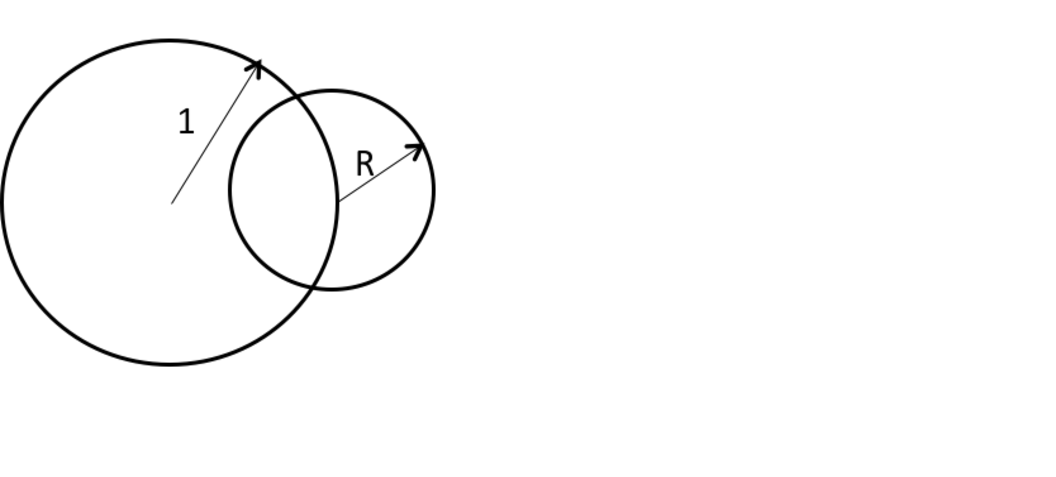
\includegraphics[width=\linewidth]{Snowman}
        \caption{Construction of Snowman molecules}
        \label{fig:snowman}
    \end{subfigure}
    \begin{subfigure}{0.5\textwidth}
        \centering
        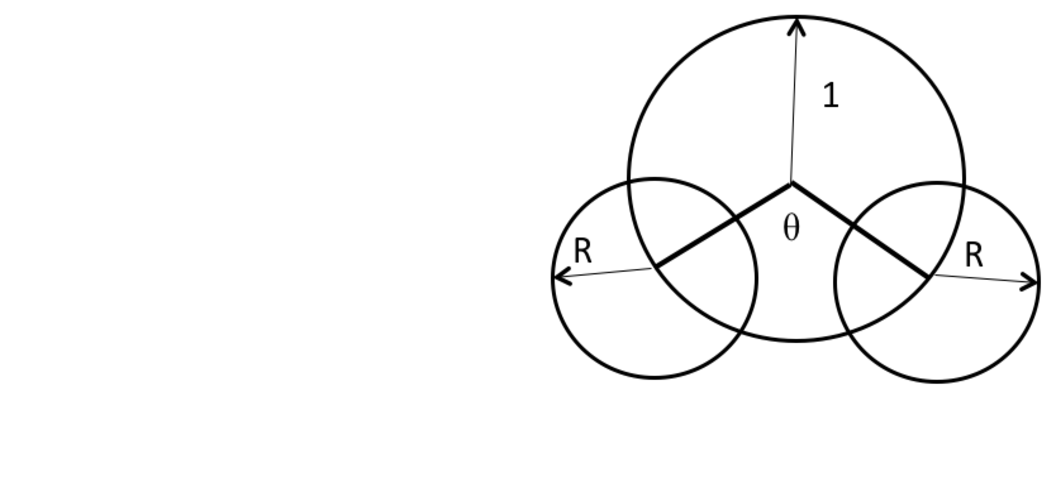
\includegraphics[width=\linewidth]{Trimer}
        \caption{Construction of Trimer molecules}
        \label{fig:trimer}
    \end{subfigure}
    \caption{Construction of the molecules used in this thesis}
    \label{fig:construction}
\end{figure}

The particles of each molecule are implemented as modified Lennard-Jones particles with $\epsilon = 1$ and $\sigma = 2r$. Interactions between combinations of particles are given by the average $r$. The bond lengths and angles use a harmonic potential with a spring constant $k=5000$, more than three orders of magnitude greater than the bonded interactions. This large spring constant is to keep the arrangement of the particles as close as possible to that of a rigid molecule.

\section{Molecular Dynamics}

The simulations in this thesis are performed using molecular dynamics, the positions of molecules are stepped through time by solving Newton's equations at each step. The software used to perform the molecular dynamics is Lammps~\tocite, an open source program designed to efficiently perform large scale molecular dynamics simulations. An integral part of the optimisation achieved by Lammps is the spatial decomposition of particles amongst the available processors, allowing for efficient use use of a large number of processors~\tocite. Spatial decomposition is a technique that divides the simulation area into a grid equal to the number of processors. Each processor is then assigned an area of the grid for which it is responsible for computing. The processors are also assigned a set of \emph{ghost particles}, particles which are outside of the region the processor is responsible for computing but are close enough to be applying a force to particles in that region. The use of ghost atoms reduces the amount of communication between processors, at each step the only communication required is the updated positions of the ghost atoms. The reduction in communication is important for efficiency as it is the major speed bottleneck in alternative methods.

Lammps implements the modified Lennard-Jones potential and also the associated reduced units.
\towrite{reduced units}

The thermodynamic ensemble for the simulation is the NPT ensemble, with a constant number of particles (N), constant pressure (P) and constant temperature (T). The constant number of particles is achieved by not adding or removing any particles from the simulation, the pressure and temperature are kept constant by a Noose-Hoover thermostat\tocheck.
\towrite{Thermostat and barostat}

\section{Units}

In a simple system like a Lennard-Jones system the standard units for various properties are cumbersome and not well matched to the specific system. Instead a set of reduced units is used, using a mass $m = 1$ as the fundamental unit. A series of further units can be derived using the parameters of the Lennard-Jones potential $\sigma$ and $\epsilon$. 

\begin{table}
    \begin{tabular}{ l c }
        Mass & $ m = 1$ \\
        Energy & $E^* = E/\epsilon$ \\
        Temperature & $T^* = T_k/\epsilon$ \\
        Length & $L^* = L/\sigma$ \\
        Pressure & $P^* = P\sigma^3/\epsilon$ \\
        Time & $t^* = t\sqrt{\epsilon/(m\sigma^2)}$
    \end{tabular}
    \caption{Reduced LJ Units}
    \label{tab:reduced units}
\end{table}

\section{Specific Implementations}

\subsection{Packing}

The initial configuration for the random packings is a grid of molecules in a random orientation with a distance between them larger such that they are unable to contact each other. From this state the molecules are allowed to compress and equilibrate at a temperature $T=5$, well above the melting point. The configuration was then equilibrated at a series of lower temperatures with a quenched configuration taken at each temperature.

\subsection{Dynamics}

The initial state of these runs was the same as for the packing, however the series of temperatures was finer. The other difference is that the system was equilibrated at each temperature, before a production run, from which data as collected was performed. As the temperature gets lower the timescale of the dynamical phenomenon gets slower, the length of the production run was longer for lower temperatures.

\subsection{Crystal Structures}

\begin{itemize}
    \item Isopointal algorithm
    \item starting from Toby's structures
    \item Converting to large unit cell, squaring the edges
    \item equilibration at low T
    \item Rahman-Parinello
\end{itemize}

\subsection{Interface Kinetics}

\begin{itemize}
    \item Start with crystal
    \item Melt half holding other half in place
    \item equilibrate at temperature
    \item Production run
\end{itemize}

\section{Minimisation Algorithms}

The algorithm commonly used to find the inherent structure is conjugate gradients\tocite. This is another algorithm focused on finding minima on a multidimensional landscape, $F(\vect x)$~\cite{shewchuk:94,hestenes:52}. In this case conjugate gradients is an iterative algorithm that will find the closest local minima in a small number of steps. The conjugate gradient algorithm is most simply explained as as extension of another iterative algorithm, steepest descent. The naming of the steepest descent algorithm is very self descriptive, a step of size $\gamma$ is taken in the direction of the steepest descent. Each step is given by
\begin{equation}
    \vect r_{i+1} = \vect r_i - \gamma \nabla F(\vect r_i)
\end{equation}
where $\vect r_i$ is the approximation to the minimum at step $i$ and
\begin{equation}
    \nabla = \left (\pddiff{}{x_1}, \pddiff{}{x_2},\cdots,\pddiff{}{x_n} \right )
\end{equation}
Steepest descent is limited in that it will often zig-zag slowly towards the minimum, requiring a large number of steps. The conjugate gradient method takes into account the direction of the previous step, with the new step being a linear combination of the previous step and the steepest descent at the current point
\begin{align}
    \vect r_{i+1} &= \vect r_{i} - \Delta \vect r_i \\
     \Delta \vect r_{i} &= \alpha( \nabla F(\vect r_i) + \beta \Delta \vect r_{i-1})
\end{align}
with constants $\alpha$ and $\beta$ which in practice are calculated each step for fastest convergence. Note that it is not possible to take a first step with the conjugate gradient algorithm, the direction of the previous step is needed. In practical applications of the conjugate gradient algorithm the initial step is taken using the steepest descent algorithm, with the remaining steps using conjugate gradient. Each step of the conjugate gradient algorithm requires more calculation than a step with the steepest descent algorithm, the improvement from using conjugate gradient comes from reducing the number of steps required~\cite{knyazev:08}.

Both the steepest descent and the conjugate gradient methods are good at finding the local minimum. Often more important than local minima are the global minima, where other techniques are required. One case where finding the global minima is important is the formation of a crystal from a liquid phase. This is one of the common techniques, known in computer science as simulated annealing~\tocite, the idea is that you start at a high temperature and slowly reduce the temperature. If the reduction in temperature is slow enough the final state will be the global minimum of the function, otherwise it will be a local minima. This is exactly the process that is being investigated in this thesis using molecular dynamics to sample the possible space of the function describing the degrees of freedom of all the molecules with the state of the function given by the total energy of the molecules. Here the aim is to arrange the molecules in the lowest energy configuration, the crystal state. In some cases, like a single component disc liquid will easily crystallise~\tocite, other cases like certain binary disc mixtures~\tocite are highly resistant to crystallisation. In these cases there are other methods to find the lowest energy state.

Molecular dynamics simulations typically have a large number of particles to give a reasonable approximation of real world phenomena and to remove the effects of particles interacting with themselves through the periodic boundary conditions. These requirements are not always the case, by exploiting the symmetry of a space group and \emph{isopointal sets} the dimensionality and search space can be dramatically reduced~\cite{hudson:10}. An isopointal set is a space group and a minimal set of symetrically distinct sites, with the rest of the molecules in the unit cell generated by application of the symmetry operations. These minimal set of sites are known an \emph{Wyckoff} sites~\cite{gelato:87,bergerhoff:99}. These simplifications reduce the dimensionality of the problem significantly, each space group has a small set of possible Wyckoff sites, each with only a few optimisation parameters which can be optimised using \emph{Monte Carlo} simulated annealing.

The basis of \emph{Monte Carlo} methods is that the space of interest is traversed stochastically. It is used in a number of applications, the simplest application of this method is to approximate the area of a region in space. This can be done by taking an easy to calculate enclosing area, like a square, and an unknown area defined by some inequalities and generating a series of points in the larger area~\figref{monte carlo pi}. The fraction of points in the unknown area is an approximation of the relative size of the area. We can also consider this process as an accept/reject criterion, accept if in the area of interest, reject if not. In this case the percentage accepted is important. In simulated annealing this accept/reject criterion is related to the energy of the state, a high energy state is less likely to be accepted than a low energy state. As the temperature is reduced the region of acceptance shrinks along with the size of the jumps between configurations, with the final configuration ideally being the lowest energy configuration.

\begin{figure}
    \centering
    \animategraphics[loop,autoplay,width=0.5\linewidth]{3}{Pi-}{0}{9}
    \caption[Approximating $\pi$ using the monte carlo method]{Approximating $\pi$ using the Monte Carlo method using the ratio of points falling in each area. Increasing the number of points reduces the error in the result.}
    \source[\ccby]{montecarlopi}
    \label{fig:monte carlo pi}
\end{figure}


